
\noindent\begin{minipage}{\textwidth}
    \begin{table}[H]
        \centering
        \caption{Hiperparâmetros e Resultados do Melhor Modelo - inception\_v12\_BR\_opt\_aug}
        \vspace{0.2cm}
        \resizebox{\textwidth}{!}{%
            \begin{tabular}{ll | lrrr}
                \hline
                \multicolumn{2}{c|}{\textbf{Hiperparâmetros}} & \multicolumn{4}{c}{\textbf{Métricas por Classe}} \\ \hline
                \textbf{Parâmetro} & \textbf{Valor} & \textbf{Classe} & \textbf{Precisão} & \textbf{Recall} & \textbf{F1-Score} \\ \hline
    Agendador (Patience) & 5 & 31.2 & 0.4266 & 0.4189 & 0.4227 \\ 
Agendador de LR & ReduceLROnPlateau & 31.3 & 0.2154 & 0.4309 & 0.2872 \\ 
Architecture & inception\_v3 & 31.4 & 0.3161 & 0.2149 & 0.2559 \\ 
Batch Size & 32 & 32.3 & 0.2063 & 0.2751 & 0.2358 \\ 
Data Augmentation & False & 32.4 & 0.0548 & 0.1111 & 0.0734 \\ 
Decaimento de Peso (WD) & 0.0000 & 33.3 & 0.2619 & 0.0509 & 0.0853 \\ 
Dropout & 0.5905 & 41.4 & 0.1176 & 0.1702 & 0.1391 \\ 
Função de Perda & CrossEntropyLoss & 41.5 & 0.2400 & 0.2791 & 0.2581 \\ 
Hidden Units & 1024 & 42.4 & 0.1176 & 0.0328 & 0.0513 \\ 
Label Smoothing & 0.1000 & 44.4 & 0.0000 & 0.0000 & 0.0000 \\ 
\cline{3-6} 
Otimizador & AdamW & \textbf{Média (Macro)} & 0.1957 & 0.1984 & 0.1809 \\ 
Taxa de Aprendizado (LR) & 2.97e-04 & \textbf{MCC} & \multicolumn{3}{c}{0.1301} \\ 
Unfreeze Layers & 6 &  & & &  \\ 
            \hline
            \end{tabular}%
        }
    \end{table}

    \begin{figure}[H]
        \centering
        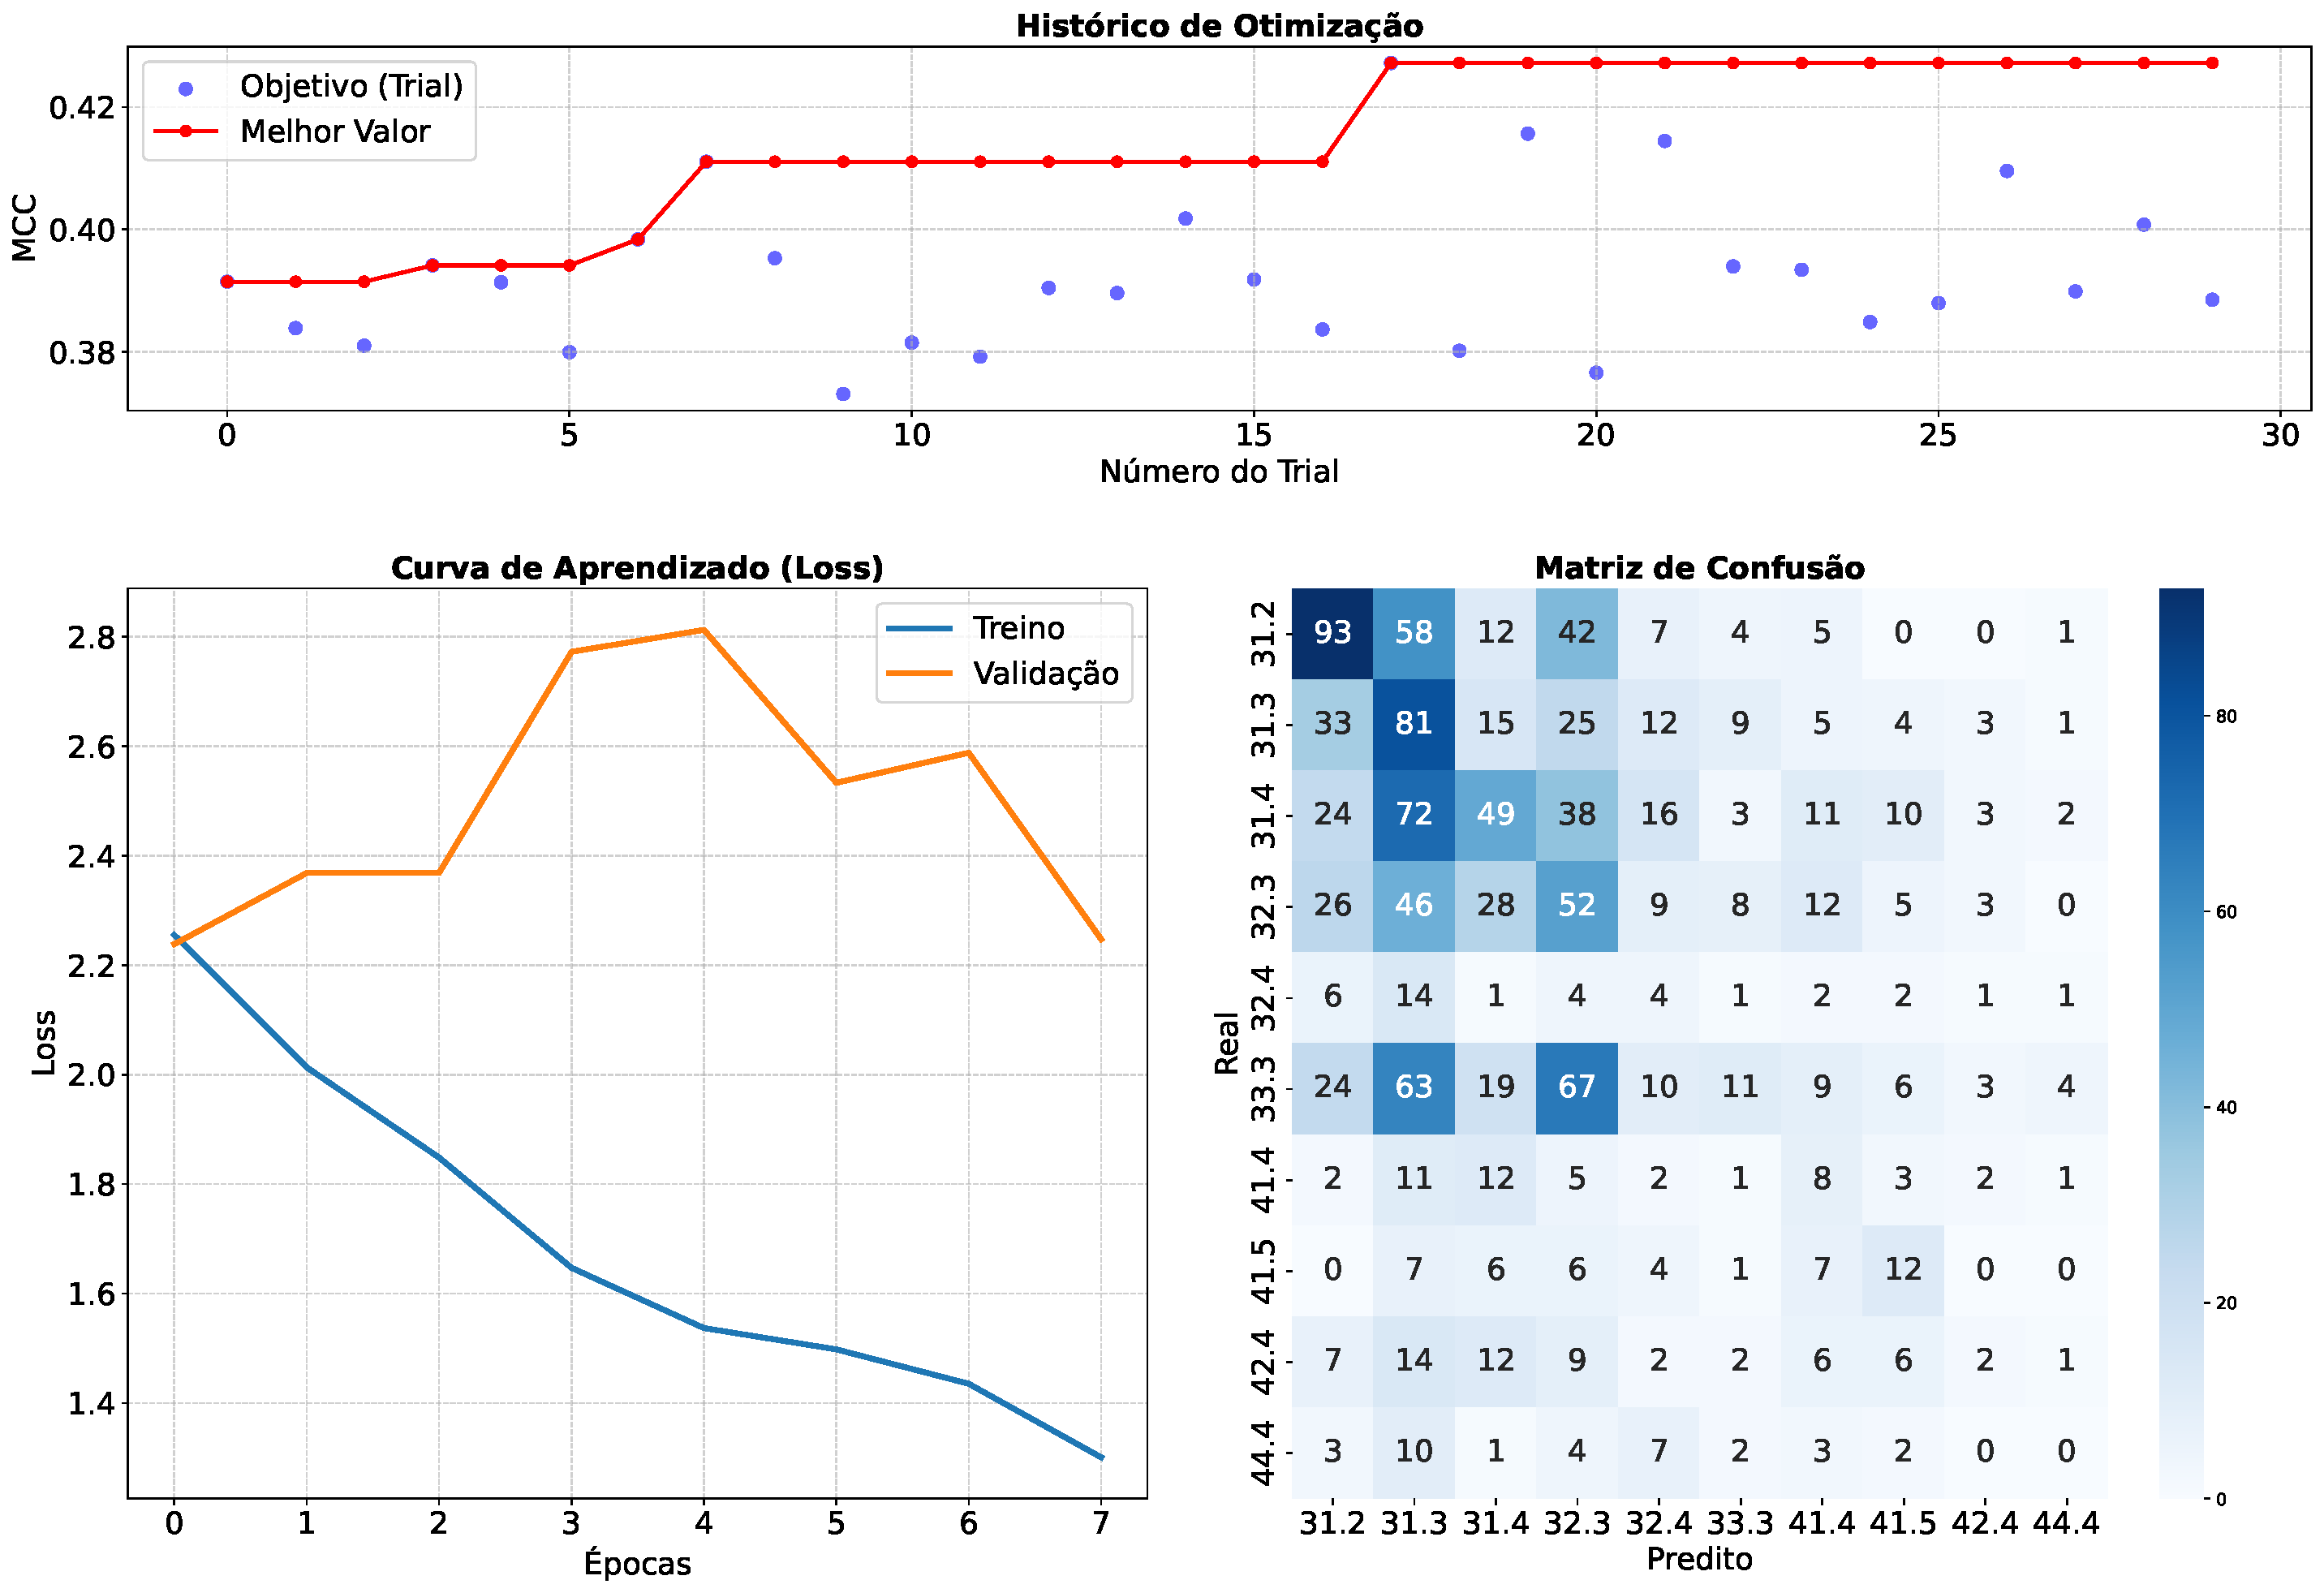
\includegraphics[width=0.85\textwidth]{tex/appendix/experiments/inception_v12_BR_opt_aug/dashboard_consolidado.pdf}
        \caption{Histórico de Otimização, Curvas de Aprendizado e Matriz de Confusão - inception\_v12\_BR\_opt\_aug}
    \end{figure}
\end{minipage}
\clearpage
